\documentclass{article}
\usepackage[utf8]{inputenc}
\pagenumbering{roman}
\usepackage[letterpaper, portrait, margin=1in]{geometry}
\usepackage{graphics} 
\usepackage{graphicx} 
\usepackage{epsfig} 
\usepackage{times} % assumes new font selection scheme installed
\usepackage[dvipsnames]{xcolor} 
\usepackage{gensymb}
\usepackage{soul}
\usepackage[hyphens]{url}
\usepackage{hyperref}
\hypersetup{breaklinks=true}
\urlstyle{same}
\usepackage[noadjust]{cite}
\widowpenalty10000
\clubpenalty10000
\usepackage[font=footnotesize]{caption}
\usepackage{subcaption}
\usepackage{wrapfig}
\usepackage[nottoc]{tocbibind}

\captionsetup[table]{justification=centerlast,
                     labelsep=newline,
                     font={small,sc}}
\captionsetup[sub]{font=footnotesize}

\begin{document}

\begin{center}
\LARGE \textbf{A Novel Neuromuscular Sensing Platform for Intuitive Control of Robotic Exoskeletons in Extravehicular Activities}
\normalsize
\break

By: Avinash Baskaran
%%%%% BEGIN RESEARCH STATEMENT HERE:
\end{center}
\section{Hypothesis}

\large Powered exoskeletons can more effectively reduce neuromuscular fatigue  when neuromuscular activity is sensed as part of the control loop.

\section{Background}
Several hours into her third six-hour spacewalk aboard the International Space Station, astronaut Sunita Williams lost control of a large electric drill, striking and disabling a portion of a nearby electrical connector. She later attributed the cause of the accident to the overwhelming reaction force of the drill on her arm and the accumulation of stress during the task:  \emph{“It's pulling my pistol grip tool to my right... the pistol grip tool actually hit an electrical connector and bent it because it had that much force coming out”}. Williams' account is reflective of the vast majority of accidents and injuries sustained by astronauts during Extravehicular Activity (EVA), and underscores a subtle underlying danger for EVA astronauts: Neuroumuscular Fatigue \cite{Madden2017TheIO}.

\begin{wrapfigure}{l}{0.59\textwidth}
  \begin{center}
    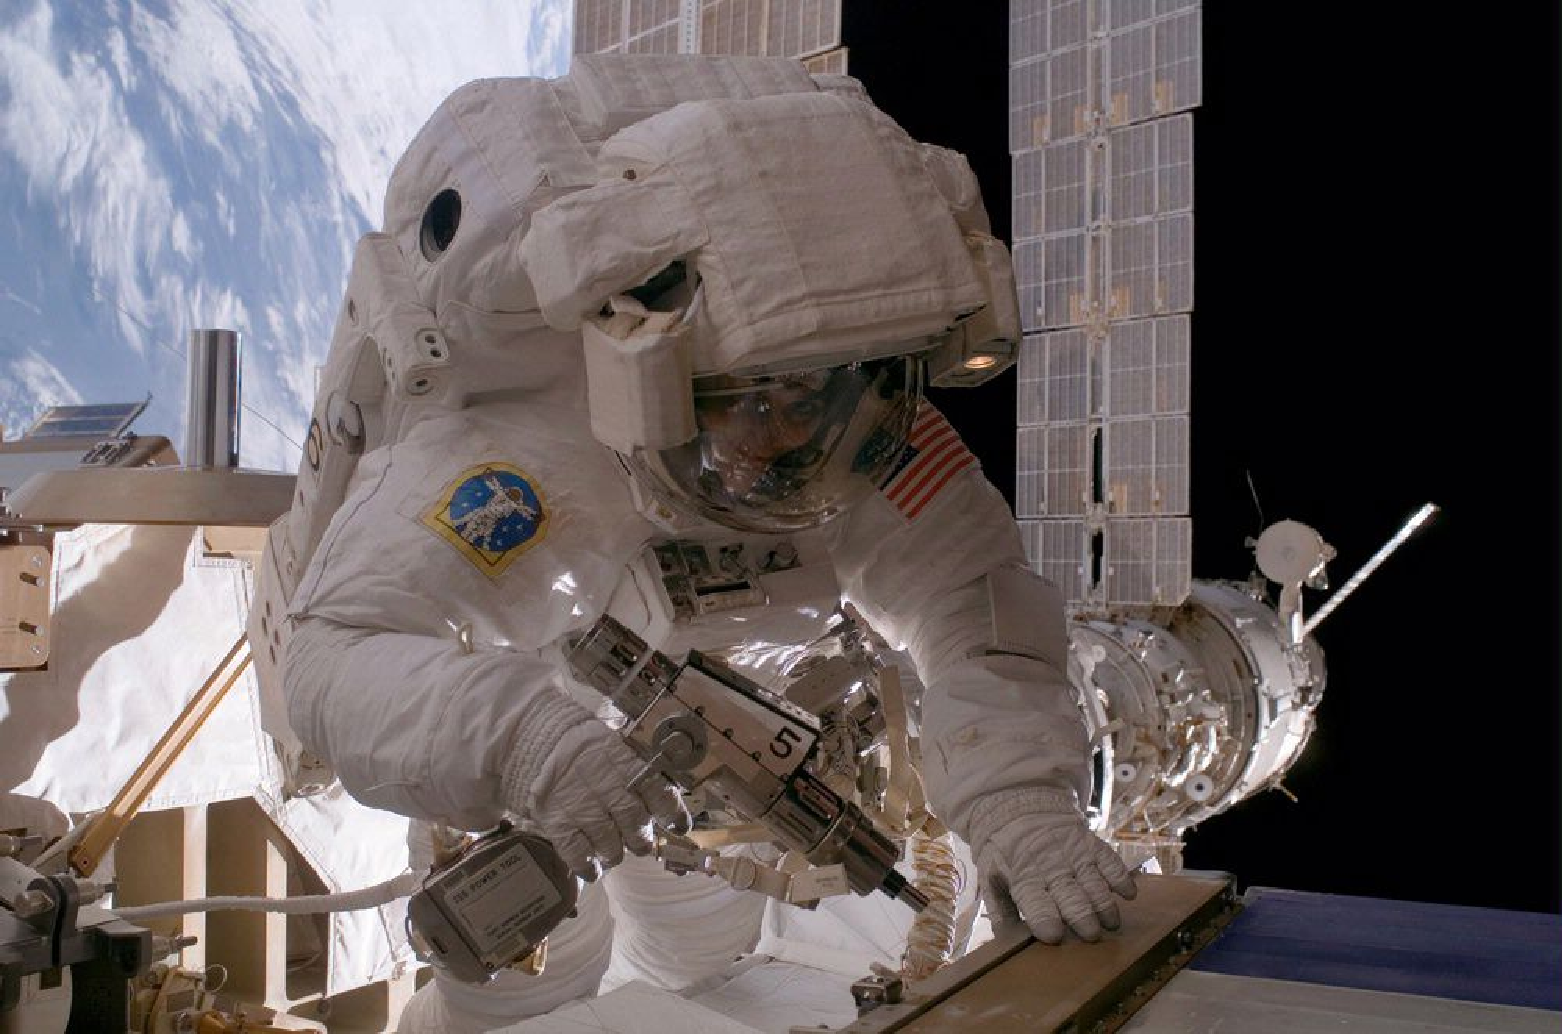
\includegraphics[width=0.59\textwidth]{figures/sunita williams pistol grip.pdf}
  \end{center}
  \caption{Astronaut Sunita Williams attempting to assemble portions of the Space Station support truss using a pistol grip tool, figure reproduced from \cite{SuniPistolGrip}}
\end{wrapfigure}

During sustained physical exercise, the intracellular excitation-contraction mechanisms used by the motor cortex to coordinate muscle activity become gradually impaired \cite{Boyas2011NMF}. This gradual impairment, called Neuromuscular Fatigue (NMF), is the result of an imperceptible delay between excitation at the motor cortex (input to the muscles) and force production (output from the muscles) that increases over the course of exercise. 

NMF-related functional deficits associated with the prolonged use of the wrist and hands, like decreased grip strength and degraded motor control, can thus arise \cite{Boyas2011NMF}. While these functional deficits usually diminish within a few hours \cite{Boyas2011NMF}, they can sometimes lead to accidents in sensitive settings, such as during surgery or during EVA task completion.

In EVA settings, NMF is amplified due to the stiffness of pressurized space suit gloves \cite{Madden2017TheIO, Rogers2017DevelopmentAT}. The stiffness of the space suit glove is dictated by life support requirements and will only increase to support human exploration in Lunar and Martian environments \cite{NASAHumanResearcherEvidenceBook}. Wearable powered assistive devices embedded in space suit gloves are among the foremost solutions being explored to help astronauts like Sunita Williams complete strenuous and dexterous EVA tasks. Such devices may be able to reduce NMF by providing targeted assistance to astronauts during EVA \cite{Madden2017TheIO}. 

\section{Previous Solutions}

\begin{wrapfigure}{0.5\textwidth}
    \centering
        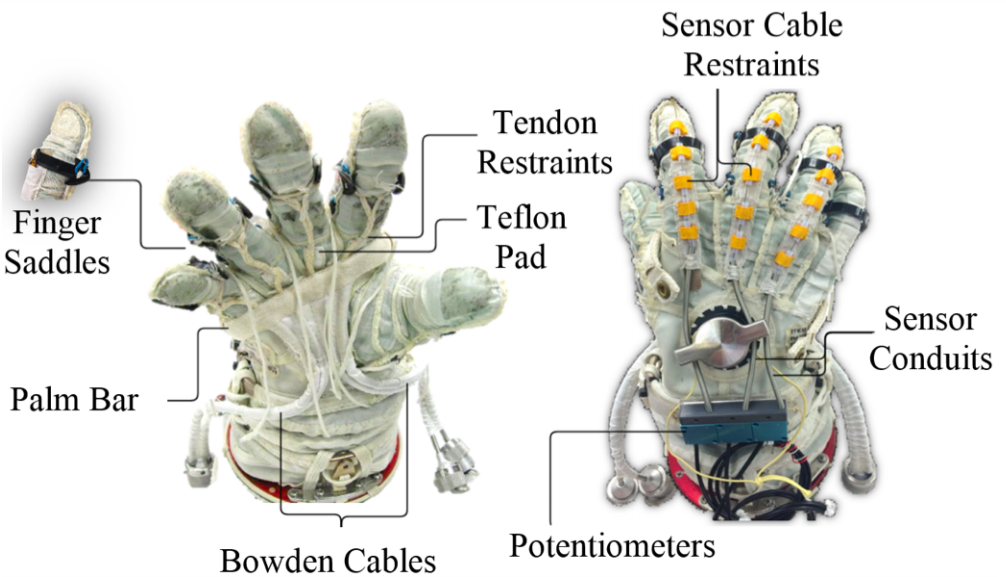
\includegraphics[width=0.5\columnwidth]{figures/SSRG1.png}
        \caption{NASA Space Suit RoboGlove (SSRG), figure reproduced from \cite{Rogers2017DevelopmentAT}}
        \label{fig:SSRG}
\end{wrapfigure}

NASA's Space Suit RoboGlove (SSRG) (fig. \ref{fig:SSRG}) is a powered exoskeleton designed to assist astronauts during EVAs \cite{Rogers2017DevelopmentAT,Madden2017TheIO, NASAHumanResearcherEvidenceBook}. The SSRG and similar devices rely on impedance or position-based sensing, responding to user kinematic action and not to neuromuscular signals. Because of this, the SSRG can't effectively measure or respond to neuromuscular artifacts like NMF and further strains the transmission of signals from the motor cortex by imposing an impedance to free movement \cite{Celik2010NormalizedMQ,Madden2017TheIO}. 

The SeptaPose Assistive and Rehabilitative (SPAR) Glove (fig. \ref{sparGlove}), successfully incorporates surface electromyography (sEMG) sensing for pose estimation and intent detection \cite{Rose2019HybridRH}. It is able to thereby respond more quickly to user intent, reducing the aforementioned impedance to free movement. However, it ignores larger neuromuscular trends and patterns, like NMF, in assistance \cite{Rose2019HybridRH}. 

\begin{wrapfigure}{0.45\textwidth}
    \centering
        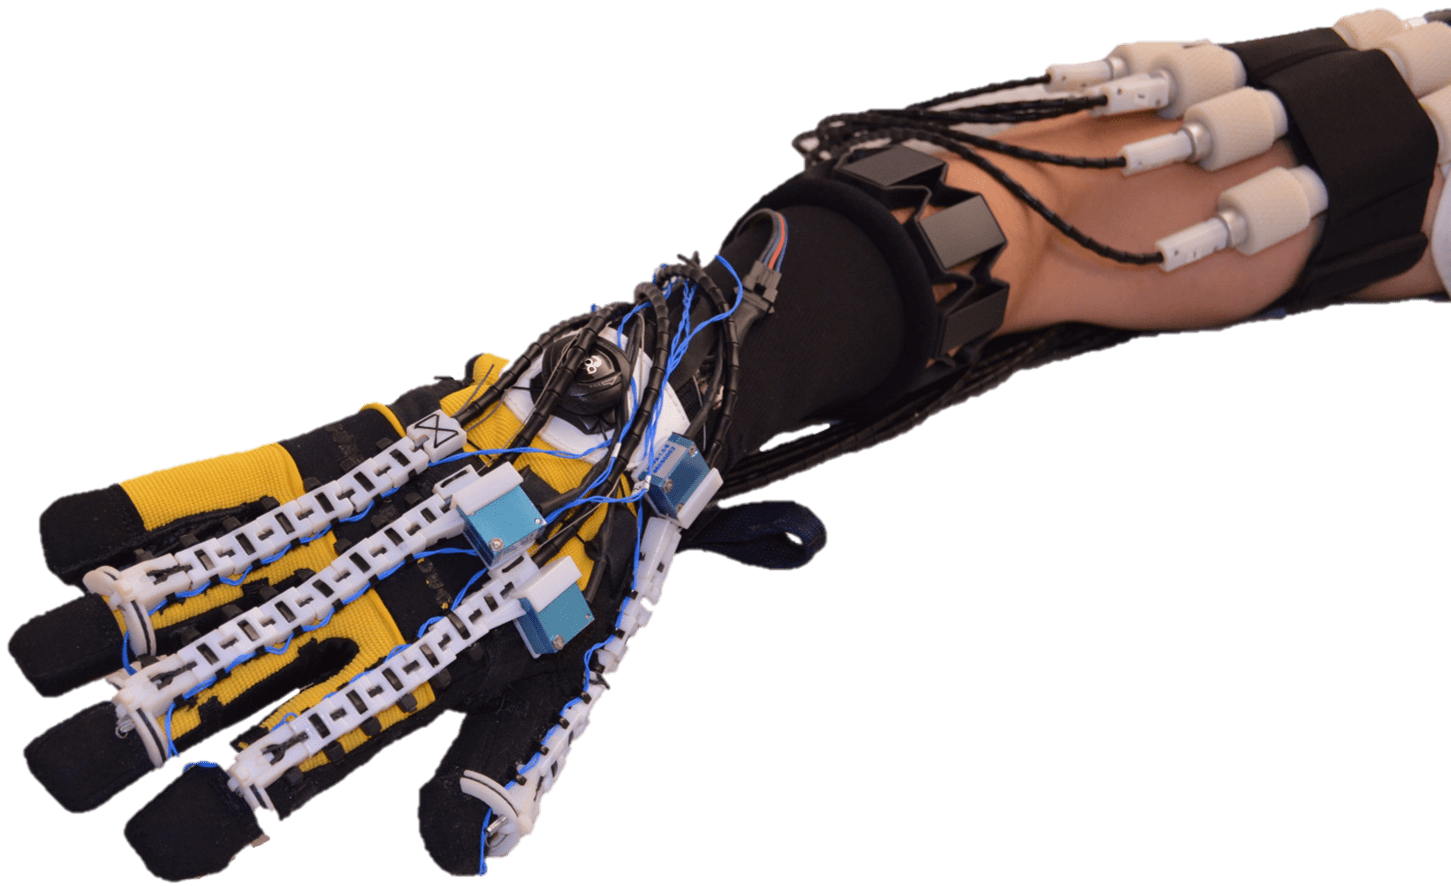
\includegraphics[width=0.42\columnwidth]{figures/SPAR_Glove_System_3-min.png}
        \caption{SeptaPose Assistive and Rehabilitative (SPAR) Glove device, figure reproduced from \cite{Rose2019HybridRH}}
        \label{sparGlove}
\end{wrapfigure}

While such devices represent a significant step towards mitigating NMF, they do not implement a targeted approach to NMF minimization such as the one described in this proposal. There remains a need for NMF pattern recognition to inform the movement of such devices so that fatigue can be efficiently and maximally reduced. Such a method would have to be designed around existing EVA suit constraints to allow free and unimpeded astronaut movement during EVAs. Without such a method, powered exoskeletons are still more of a liability than an asset in EVA settings, and astronaut NMF will remain an essentially unmanaged degree of freedom during EVAs.

\section{Proposed Research}

\textbf{\emph{I propose a novel EVA-suit compatible passive wearable device that can detect and model NMF during periods of physical activity and adjust exoskeleton response to minimize NMF.}}\\

I will develop a low-cost instrumented glove with sEMG and kinematic sensors mounted upon flexible 3d-printed sensor hubs developed by Curtis Hill at NASA's Marshall Space Flight Center \cite{CurtisHillFlexible2020}. The device will sense and analyze user NMF by measuring muscle contraction consistency, efficiency, and motor automaticity \cite{Celik2010NormalizedMQ} and communicate control instructions to powered exoskeletons. It will thus quantify neuromuscular ‘inputs’ in context with kinematic ‘outputs’ to optimize exoskeleton assistance. The device will be made suitable to existing space suit architecture to allow comfortable, efficient and effective human-robot collaborative manipulation during EVAs.

\section{Research Plan}
\subsection{Year 1: Design and Construction} 
The proposed device must meet certain functional requirements: It must be able to sense neuromuscular signals, use these signals to quantify NMF, and modulate exoskeleton assistance accordingly. The device must further be flexible, comfortable and non-intrusive to be useful in EVA settings.

To achieve these functional requisites, the device will include multiple commercial off-the-shelf sEMG, accelerometer and gyroscope sensors, a microprocessor, and a system for data transmission. The proposed glove will be composed of a lightweight lycra fabric mesh with flexible sensor hubs per Hill et. al. \cite{CurtisHillFlexible2020} which will ensure minimal accumulation of heat and moisture. The commercial off-the-shelf (CoTS) sensors will be affixed to the glove at flexible sensor hubs produced in collaboration with Curtis Hill at NASA's Marshall Space Flight Center (MSFC), who communicated his interest in supporting my extramural experience. The sensor hubs will be secured at the dorsal wrist, hand, and upper arm with embedded wiring for power and data transmission.

A microcontroller mounted on the glove will be used to collect and analyze sEMG sensor data in real time, in both the frequency and time domain. The controller will build and update a power spectrum of the data using a 6th order autoregressive model using incoming sEMG data \cite{Madden2017TheIO}. The model will be concurrently develop a time series formulation of median response frequencies (MF) with which the controller will continually perform a least-squares regression to quantitatively describe user NMF \cite{Madden2017TheIO}. Further time series analysis of the sEMG output and MF model will be used to assess factors including movement fractionation and spasticity, as well as muscle contraction features like consistency, efficiency, latency, and motor automaticity \cite{Celik2010NormalizedMQ, Min2018ElectromyogramRU} to inform NMF estimation. Kinematic outputs including wrist and hand segment movement in the flexion/extension direction and adduction/abduction direction will be used to estimate intended hand movement \cite{Safavynia2011MuscleSI,Rose2019HybridRH}. Together, the sEMG and kinematic data will be used to predict trends in user NMF, and command exoskeleton assistance to minimize latency, effort and fatigue.

\begin{wrapfigure}{2}{0.5275\textwidth}
  \begin{center}
    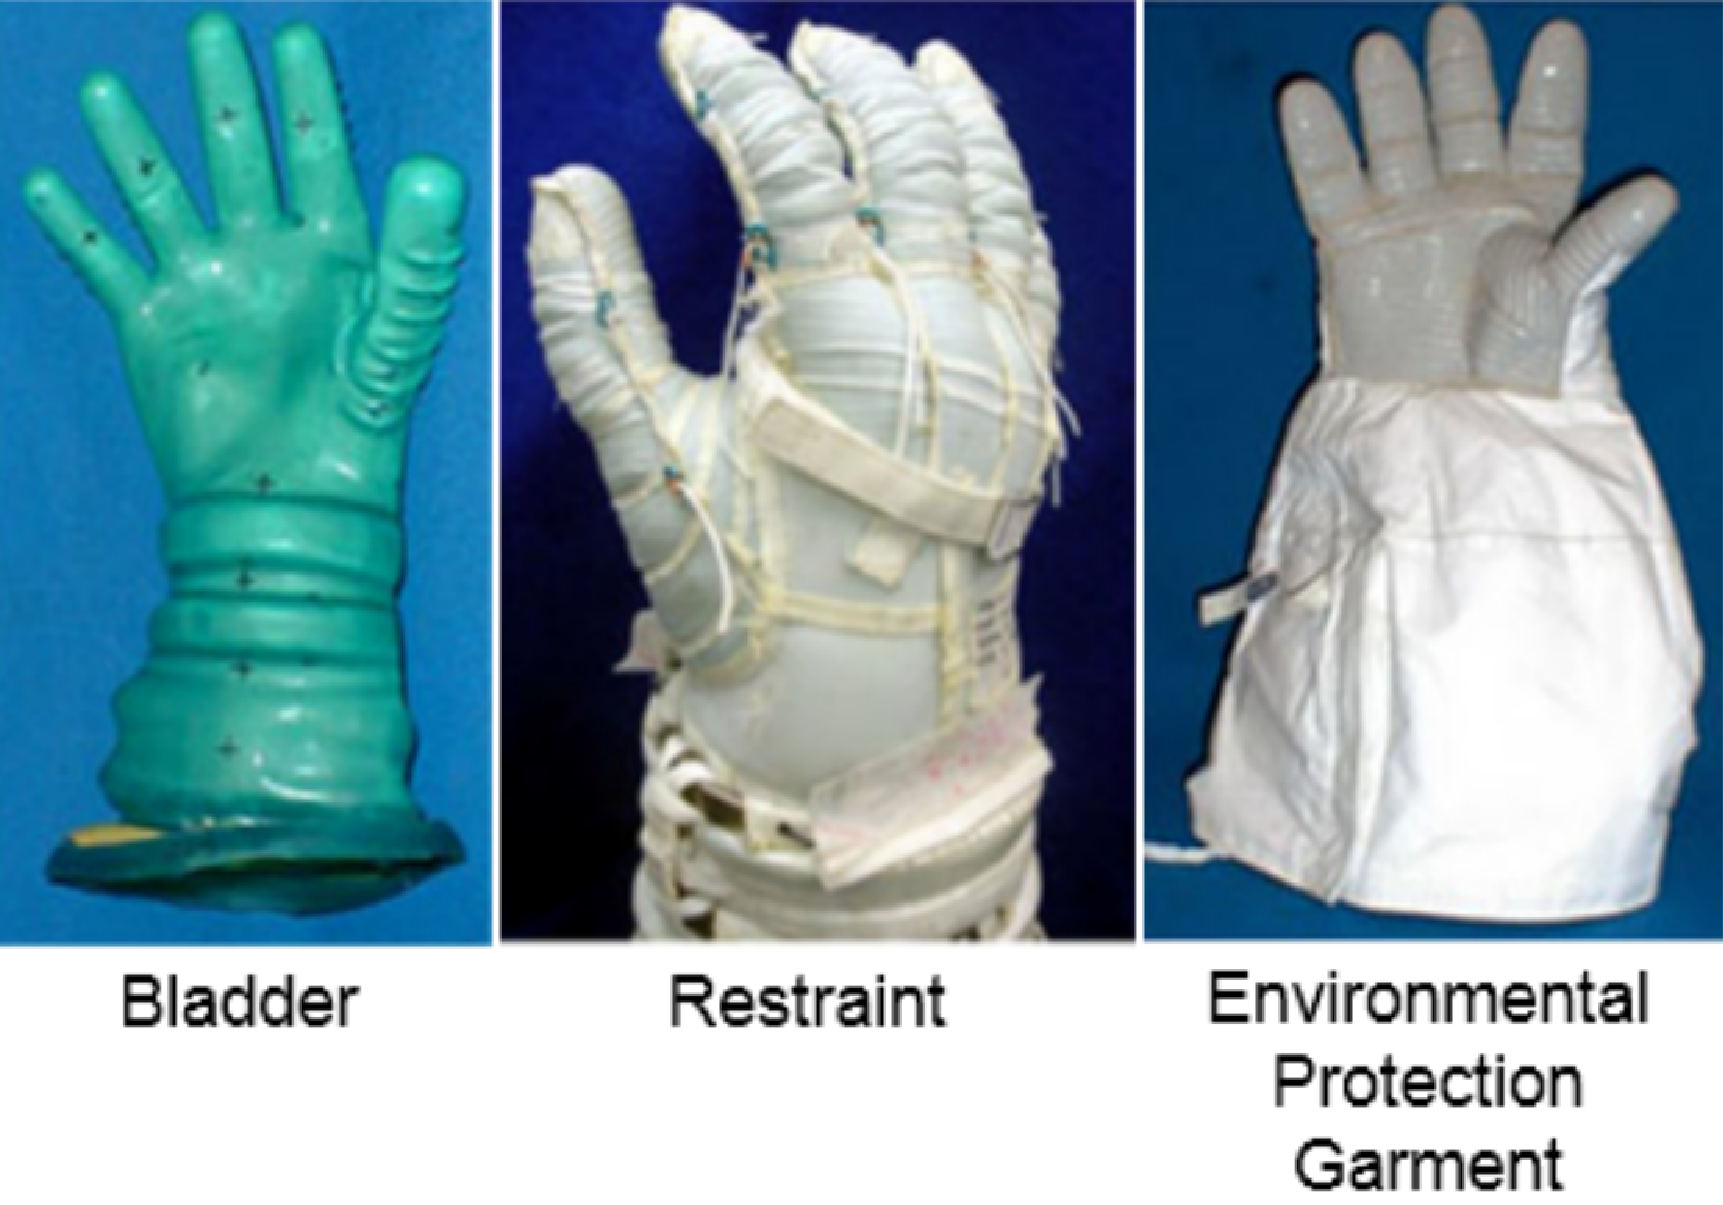
\includegraphics[width=0.5275\textwidth]{figures/space suit glove design 2.pdf}
  \end{center}
  \caption{Space Suit glove architecture, figure reproduced from \cite{Rogers2017DevelopmentAT}}
  \label{SpaceSuitLayers}
\end{wrapfigure}

To comply with the space suit design constraints, Powered exoskeletons designed for EVA use must be attached at the restraint layer of the space suit glove above the Bladder layer (shown in fig. \ref{SpaceSuitLayers}) so that the space suit's internal pressure is preserved. However, the proposed instrumented glove must be worn under the bladder layer for electromyographic transduction. Thus, it must communicate to the exoskeleton across the bladder layer wirelessly. The environmental protection garment (fig. \ref{SpaceSuitLayers}) is largely radiopaque, such that the internal volume of the space suit can support radio communication with minimal losses and without interfering with other communication systems \cite{Taj-Eldin:2015}. A self-shielded wireless body area radio communication protocol that was previously developed for intra-spacesuit sensing \cite{Taj-Eldin:2015} will be adopted into this research to allow the proposed device to be incorporated into the existing Phase VI EVA glove architecture with a minimal physical and electromagnetic presence \cite{Madden2017TheIO}.

%%%% Wireless optical communication (WOC) data transmission have been explored for use in nonstandard environments, including underwater and space environments, and can offer numerous advantages to other data transmission methods due to it offers bandwidth that is several orders of magnitude higher The instrumented glove will be worn in contact with the skin, but will include outward facing LEDs. Control instructions generated by the microcontroller will be transmitted via high frequency LED pulses \cite{Takai2014OpticalVC} across the semi-translucent bladder without affecting its structural integrity. Photoresistors connected to a secondary microcontroller on the restraint layer will be used to process the ODT signals and control exoskeleton actuators as mentioned previously.

\subsection{Year 2: Validation} 

If funded, year two of this research will be spent evaluating whether the proposed system can achieve statistically significant NMF reduction during intense physical activity.

Twenty human participants will be recruited and asked to perform a series of exercises while wearing the SPAR Glove exoskeleton (fig. \ref{sparGlove}) \cite{Rose2019HybridRH} surrounded by a loose-fitting radiopaque textile \cite{Taj-Eldin:2015} to emulate the radio shielding of the bladder layer of the space suit glove. Beneath the exoskeleton, a thick rubber glove will be worn separating it from the instrumented glove, which will be worn in contact with the skin. A defined workspace will be used with the arms in a neutral posture \cite{Madden2017TheIO, Rogers2017DevelopmentAT}.
%%%%%%%%%%%%

%%% CAD???

%%%%%%%%%%%%

Each participant will be first asked to perform 5 maximum voluntary contractions (MVCs) of the hand while holding a hand dynamometer. This measurement will be used to develop a threshold value of 20\% MVC strength. They will then be asked to perform am isometric constant force grip for ten seconds, immediately followed by a cyclic gripping task for 60 seconds. This set will be repeated 5 times with 5 minute breaks between sets, while the subject is holding the hand dynamometer and receiving visual feedback to maintain the threshold force \cite{Madden2017TheIO}. The tasks will be performed firstly with exoskeleton powered off. After a break period of 24 hours, they will be asked to perform the tasks while receiving assistance per the SPAR Glove's native control architecture \cite{Rose2019HybridRH}. After a third break period, they will be asked to perform the task while receiving assistance from the SPAR Glove with feedback from the instrumented glove. This experimental protocol is designed to assess whether feedback from the instrumented glove can allow an exoskeleton to reduce NMF by at least 10\% as compared to its function without feedback, and by at least 20\% as compared with no assistance. Secondly, it will allow a validation of the proposed radio communication protocol within the radiopaque glove housing.

\subsection{Optimization} If funded, year 3 will be spent optimizing the device for simple, robust manufacturing using 3D printing technology, ensuring its high sensitivity to NMF, and validating its ease of use in EVA environments.

Single pairs of sEMG electrodes are used to establish the device design in year one. However, a single pair of surface electrodes localized over a target muscle has been shown to result in noisy, non-robust data \cite{Min2018ElectromyogramRU}. Principle components analysis (PCA) will be used to adjust the number of electrodes over each targeted muscle and identify the minimally redundant number of electrodes needed to achieve the greatest sensitivity and accuracy in NMF measurement.

Further, whereas in year one CoTS sensors are adhered to a prefabricated flexible sensor hub, in year 3, a custom flexible sensor hub with printed circuit designs for integrated inertial measurement sensing units and sEMG electrodes will be produced. This repeatable, customized sensor hub design can be be quickly and easily manufactured \cite{CurtisHillFlexible2020} with all requisite sensors built onto the flexible board. Work already completed by Curtis Hill et. al. at NASA MSFC \cite{CurtisHillFlexible2020} will thus allow for decreased manufacturing cost and increased the structural integrity of the device. 

Finally, validation testing will again be carried out, whereby 5-6 human participants will be recruited to re-evaluate the functionality of the device. A phase VI EVA space suit glove will be used in place of the simulated space glove layers to provide more robust and accurate depiction of EVA task completion. During this testing procedure, not only will gripping performance be studied, but the effect of the instrumented glove on fine motor skill completion while wearing the space suit glove will evaluated through dexterous tasks like knot tying \cite{Rogers2017DevelopmentAT}.

\section{Institutional Support} In this research, I will consult as a visiting technologist with NASA researchers and engineers at the NASA MSFC in Huntsville, AL. I have received confirmation from Curtis Hill, a researcher among the Jacobs Engineering and Science Services and Skills Augmentation Group at the MSFC, of his interest in hosting my extramural experience. Hill et. al.'s recent work in the development of flexible sensors is well-aligned with the development of the textile-based surface electrodes intrinsic to the device I propose to construct. 

Working on-site at MSFC with field experts will be vital not only to success in the project, but will also equip me as a researcher with field-specific knowledge and a robust first hand experience with the design principles guiding the development of assistive robotic systems for space exploration. Institutional collaboration with Auburn’s VCOM medical center can support participant recruitment for experimental trials using the device. I will further consult with faculty at my graduate program at Auburn University, including Dr. Pradeep Lall, with expertise in wearable sensors, Dr. David Bevly, with experience in sensor fusion methods for biomechanical analysis and Dr. Chad Rose, my PhD advisor and an expert in wearable robotics for rehabilitation.

\section{Conclusion} The immediate benefits of this research in EVA task efficiency and the enhancement of human health and performance during space exploration are in support of NASA Technology area TX04.4.1, Multi-Modal and Proximate (human-robot) Interaction. NASA's Technology Area Strategic Roadmap explicates specific research area goals including achieving practical utility for powered assistive devices like the SSRG and the SPAR Glove. The proposed research will support the realization of these and other goals and is thereby consistent with NASA's research priorities and timeline.

The proposed device also provides far-reaching applications in every area of space exploration technology. It is known that as the human body adjusts to microgravity, the central nervous system modifies muscle coordination patterns to equilibrate and maximize kinematic efficiency \cite{Massion1992StrategyAS}. The proposed instrumented glove can thus be used to inform future exoskeleton mechanical design and control system implementations to account for modified neuromuscular processes in space. The information it can provide on changes in astronauts’ neuromuscular patterns can also inform individualized exercise practice and movement therapies to best maintain muscle and bone density in microgravity. The successful completion of this project will motivate similar approaches in lower limb exoskeletons as well, which will become increasingly necessary for long term habitation in orbit and in Lunar and Martian environments.

While advancing assistive robotics for space exploration, the proposed device will also provide a low-cost and robust platform for neuromuscular analysis in terrestrial applications including augmentation of functional dexterity in surgical assistance/training, therapeutic rehabilitation for patients with neuromuscular disease and assistance for individuals with chronic musculoskeletal impairment \cite{Rose2019HybridRH}. The proposed device will provide more optimal control of exoskeletons for such applications through NMF-based performance optimization. The proposed device would thus be tremendously impactful in developing novel, individualized assistance and therapies for patients with neuromuscular diseases and UE impairment \cite{Rose2019HybridRH,Overduin2008ModulationOM}. This research and the support of the Alabama Space Grant Consortium Fellowship program will enable me to pursue the development of health technology that will enable and support long-term human presence in space.

{\footnotesize
\bibliographystyle{abbrv}
\bibliography{references}}

\end{document}
